\documentclass[12pt]{article}
\usepackage[margin=2.5cm]{geometry}
\usepackage{enumerate}
\usepackage{amsfonts}
\usepackage{amsmath}
\usepackage{fancyhdr}
\usepackage{amsmath}
\usepackage{amssymb}
\usepackage{amsthm}
\usepackage{mdframed}
\usepackage{graphicx}
\usepackage{subcaption}
\usepackage{adjustbox}
\usepackage{listings}
\usepackage{xcolor}
\usepackage{booktabs}
\usepackage[utf]{kotex}
\usepackage{hyperref}

\definecolor{codegreen}{rgb}{0,0.6,0}
\definecolor{codegray}{rgb}{0.5,0.5,0.5}
\definecolor{codepurple}{rgb}{0.58,0,0.82}
\definecolor{backcolour}{rgb}{0.95,0.95,0.92}

\lstdefinestyle{mystyle}{
    backgroundcolor=\color{backcolour},
    commentstyle=\color{codegreen},
    keywordstyle=\color{magenta},
    numberstyle=\tiny\color{codegray},
    stringstyle=\color{codepurple},
    basicstyle=\ttfamily\footnotesize,
    breakatwhitespace=false,
    breaklines=true,
    captionpos=b,
    keepspaces=true,
    numbers=left,
    numbersep=5pt,
    showspaces=false,
    showstringspaces=false,
    showtabs=false,
    tabsize=1
}

\lstset{style=mystyle}

\pagestyle{fancy}
\renewcommand{\headrulewidth}{0.4pt}
\lhead{Team Treehouse}
\rhead{Reporting with SQL Part 2 Notes}

\begin{document}
\title{Reporting with SQL Part 2 Notes}
\author{Team Treehouse}
\maketitle

\bigskip

\section{What Are Functions?}

\bigskip

\begin{itemize}
    \item Prsents data differently through manipulation
    \item \textbf{Syntax:} \textit{function name}(\textit{value or column})
    \item e.g. LENGTH(), UPPER("Andrew Chalkley"), SUM()
\end{itemize}

\bigskip

\section{Adding Text Columns Together}

\bigskip

\begin{itemize}
    \item \textbf{Snytax:} SELECT \textit{value or column} \textbar \textbar \textit{value or column} \textbar \textbar \textit{value or column}  FROM \textit{table name};
    \item \textbar \textbar $\to$ concat operator
    \bigskip

    \underline{\textbf{Example:}}

    \bigskip

    \begin{lstlisting}[language=SQL]
    SELECT first_name || " " || last_name AS "Full Name",
            email AS "Email", phone AS "Phone"
            FROM customers;
    \end{lstlisting}

    \bigskip

    \begin{center}
    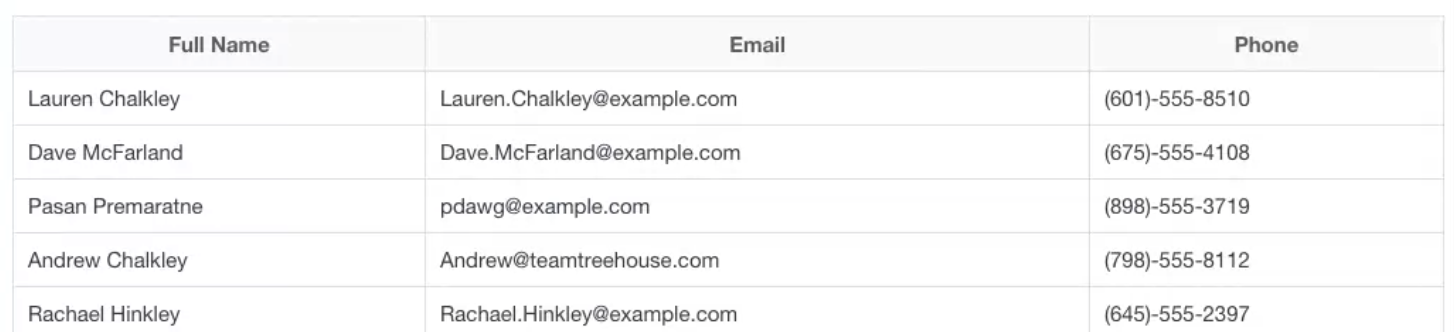
\includegraphics[width=\linewidth]{images/part_2_notes_1.png}
    \end{center}

\end{itemize}

\bigskip

\section{Single vs Double Quotes}

\bigskip

\begin{itemize}
    \item Exists difference in use
    \item Single Quote $\to$ for string literlas (e.g. 'lbs')
    \item Double Quote $\to$ for column aliases (e.g. "Max Weight")

    \bigskip

    \underline{\textbf{Example:}}

    \bigskip

    \begin{lstlisting}[language=SQL]
    SELECT maximum_weight || 'lbs' AS "Max Weight" FROM ELEVATOR_DATA;
    \end{lstlisting}

\end{itemize}

\bigskip

\section{Exercise 1}

\bigskip

\begin{itemize}
    \item Solution included in \textit{exercise\_1.sql}
\end{itemize}

\bigskip

\section{Finding the Length of Text}

\bigskip

\begin{itemize}
    \item \textbf{Syntax:} SELECT LENGTH(\textit{value or column}) FROM \textit{table name};
    \item Returns length of a value or value in each row of a column
    \item Can also be used in WHERE
    \begin{itemize}
        \item \textbf{Syntax:} SELECT \textit{columns} FROM \textit{table name} WHERE LENGTH(\textit{column name}) \textit{operator} \textit{value};
    \end{itemize}

    \bigskip

    \underline{\textbf{Example:}}

    \bigskip

    \begin{lstlisting}[language=SQL]
    SELECT username, LENGTH(username) AS "length" from customers ORDER BY length DESC LIMIT 1;


    SELECT username FROM customers WHERE LENGTH(username) < 7;


    SELECT username LENGTH(username) AS "length" FROM customers WHERE length < 7;
    \end{lstlisting}

    \bigskip

    \begin{center}
    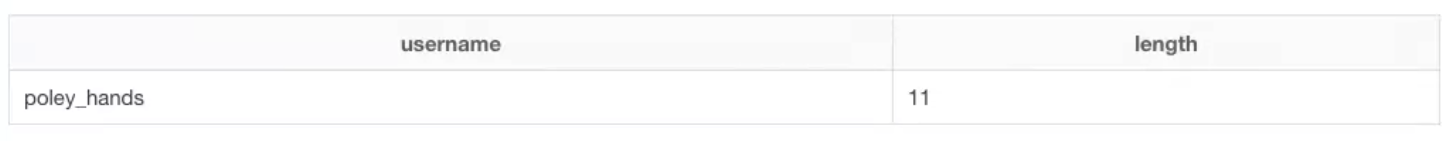
\includegraphics[width=\linewidth]{images/part_2_notes_2.png}
    \end{center}

\end{itemize}

\bigskip

\section{Exercise 2}

\bigskip

\begin{itemize}
    \item Solution included in \textit{exercise\_2.sql}
\end{itemize}

\bigskip

\section{Changing the Case of Text Columns}

\bigskip

\begin{itemize}
    \item \textbf{Syntax (Upper):} SELECT UPPER(\textit{value or column}) FROM \textit{table name};
    \item \textbf{Syntax (Lower):} SELECT LOWER(\textit{value or column}) FROM \textit{table name};
    \item Returns values in a column in upper or lower case
    \item Search can be made case insensitive
    \begin{itemize}
        \item SELECT \textit{column} FROM \textit{table name} WHERE LOWER(\textit{column name}) = \textit{value in lowercase};
    \end{itemize}

    \bigskip

    \underline{\textbf{Example:}}

    \bigskip

    \begin{lstlisting}[language=SQL]
    SELECT * FROM customers WHERE LOWER(email) = "andrew@teamtreehouse.com";
    \end{lstlisting}

\end{itemize}

\bigskip

\section{Exercise 3}

\bigskip

\begin{itemize}
    \item Solution included in \textit{exercise\_3.sql}
\end{itemize}

\bigskip

\section{Creating Excerpts From Text}

\bigskip

\begin{itemize}
    \item SUBSTR
    \begin{itemize}
        \item \textbf{Syntax:} SELECT SUBSTR( \textit{value or column}, \textit{start}, \textit{length}) FROM \textit{table name};
        \item Allows to create ellipsis
        \begin{itemize}
            \item Prevents website from being overloaded with details
        \end{itemize}

        \bigskip

        \underline{\textbf{Example:}}

        \bigskip

    \begin{lstlisting}[language=SQL]
    SELECT name SUBSTR(description, 1, 50) || "..." AS short_description, price FROM products;
    \end{lstlisting}

    \end{itemize}
\end{itemize}

\bigskip

\section{Exericse 4}

\bigskip

\begin{itemize}
    \item Solution included in \textit{exercise\_4.sql}
\end{itemize}

\bigskip

\section{Replacing Portions of Text}

\bigskip

\begin{itemize}
    \item \textbf{Syntax:} SELECT REPLACE(\textit{original value or column name}, \textit{target string}, \textit{replacement string}) FROM \textit{table name};
\end{itemize}


\end{document}